\newcommand{\COMMENT}[1]{\noindent\fbox{\parbox{0.98\linewidth}{\bfseries #1}}}


\chapter{Fundamentação Teórica}
\label{ch:fundamentos}

Neste capítulo são fundamentados os conceitos necessários para o entendimento da proposta e do funcionamento do protocolo. Na Seção \ref{sec:microsservicos} é definido o que são microsserviços e conceitos relacionados à sua arquitetura, assim como o processo de criação de um contrato e as possibilidades de provedores e serviços. Na Seção \ref{sec:blockchain} é definido o conceito de \textit{Blockchain}, seu funcionamento, formas das redes e de consenso, a arquitetura das transações e as carteiras digitais. Na seção \ref{sec:blockchain:smart_contracts} aborda-se o conceito de contratos inteligentes em tecnologias de \textit{Blockchain} disponíveis no mercado.


\section{Provisionamento e gerenciamento de microsserviços}
\label{sec:microsservicos}

Os microsserviços podem ser caracterizados como um modelo de arquitetura orientada a serviços, representando pequenas partes do sistema que funcionam independentemente e realizam suas funções da mesma forma. Nesse âmbito, o processo de interconexão e união dos microsserviços - que é fundamentalmente responsável pela execução correta do sistema resultante como um todo - é realizado através de troca de mensagens pela rede \cite{microsservicos:newman_microsservicos}.
%
Tomando o rumo de outra possível definição, os microsserviços tratam-se um conjunto de elementos fracamente acoplados com contextos limitados. Essas duas características elencadas são significativas para o correto desenvolvimento da arquitetura. 
%
A primeira define que os microsserviços, por funcionarem de maneira independente, podem também ser atualizados individualmente sem que haja problemas na aplicação ou na comunicação do microsserviço atualizado em questão com os outros.
%
A segunda característica diz respeito ao fato de que ao desenvolver um microsserviço não há necessidade de conhecer ou mesmo preocupar-se com o funcionamento interno, estruturas e bancos de dados, versão ou outras informações específicas dos outros microsserviços cujos quais este se comunica \cite{microsservicos:netflix}. As únicas informações alheias necessárias para o funcionamento são as relativas exclusivamente ao processo de comunicação em si, como formato dos dados de envio e recebimento assim como das requisições e respostas.
%
Geralmente o processo de comunicação entre diferentes microsserviços é feito por meio de \acp{API}, corroborando com o que é proposto pela arquitetura e facilitando o quesito de independência entre as partes \cite{microsservicos:newman_microsservicos, microsservicos:empresas}.

As vantagens trazidas pela arquitetura de microsserviços, quando comparadas com o modelo monolítico, são vastas graças as características fundamentais dos mesmos e da organização distribuída em si.
%
De modo geral, o desenvolvimento pode ser melhor regido pois há possibilidade de designar equipes específicas para a construção  de microsserviços.
%
O controle de código melhora do ponto de vista de organização, pois ao invés de um grande bloco compartilhado há partes menores divididas coexistindo remotamente. Tal fato facilita o processo de programação, porém cria novos desafios de integração e coordenação das partes. 
%
O versionamento é simplificado uma vez que os microsserviços podem ser atualizados individualmente sem afetar o funcionamento ou estabilidade da aplicação como um todo \cite{microsservicos:artigo_microsservicos}. Em casos de problemas é simples retornar um microsserviço para uma versão anterior sem comprometer as outras partes do sistema ainda operando em versões anteriores, bem como a comunicação com elas \cite{microsservicos:newman_microsservicos}.

%
A dinamicidade do sistema em geral também aumenta, pois graças a característica de individualidade dos microsserviços é possível adotar diferentes tecnologias que se adaptem melhor às necessidades de funcionamento e objetivos de cada um.
%
Da mesma forma podem também ser adotadas novas tecnologias mais facilmente, pois os custos e riscos para tal inovação são reduzidos ao alterarmos apenas partes pequenas e independentes do código. 
%
Por fim uma das maiores vantagens da arquitetura é a escalabilidade que tem um potencial maior com pequenos serviços e não depende de  gargalos operacionais relacionados à aplicações monolíticas. A distribuição de recursos computacionais pode ainda ser feita de maneira personalizada, de modo que os microsserviços com uma carga de trabalho maior ou que tem mais requisições tenham à sua disposição mais processamento, armazenamento, uma banda maior e etc.


\subsection{Ciclo de vida}

Os microsserviços, como já mencionado, funcionam de maneira distribuída podendo assim ser executados individualmente e em diferentes máquinas e ainda assim compor a aplicação. Portanto muitas empresas que adotam a tecnologia dos microsserviços utilizam também de serviços de provedores \ac{IaaS} de terceiros para melhorar o desempenho, reduzir custos e necessitar de menos hardware próprio \cite{microsservicos:empresas}. O processo de provisionamento dos microsserviços, sobretudo quando hospedados em nuvens ou em provedores nas bordas da Internet, assim como qualquer sistema distribuído provisionado em ambientes virtualizados, pode ser desmembrado em cinco etapas \cite{nuvem_sla:tese_guilherme}: 

 
 \begin{itemize}
     \item \textbf{Especificação:}
        No processo de especificação são definidas quais serão as necessidades do cliente para o funcionamento efetivo dos microsserviços na infraestrutura contratada. Características físicas como modelo de processadores, número de núcleos, memória, disco bem como sistema e aplicações das máquinas destino são tratadas nesse processo. O protocolo proposto no presente trabalho (\ref{ch:proposta}) trata esta parte no campo de mensagens de requisição de alocação. Estas ficam retidas na cadeia após o consenso para registro do processo contratual com o provedor e das informações referentes às configurações solicitadas.
     \item \textbf{Escalonamento:}
        Na fase de escalonamento são associadas as requisições dos clientes com os respectivos provedores. Os recursos solicitados são também agrupados ou divididos em zonas, regiões e domínios de acordo com a necessidade do cliente ou disponibilidade do provedor para tal. O protocolo nessa parte é responsável por armazenar as respostas do servidor relacionadas a como o escalonamento foi feito e como estão distribuídas as máquinas alocadas de modo que essas informações fiquem armazenadas e visíveis para o cliente. Alterações na alocação também podem ser informadas em tempo real através das mensagens para atualização de dados e manutenção de um histórico de mudanças.
     \item \textbf{Execução:}
        A fase de execução acontece após as duas anteriores e, intuitivamente, refere-se ao processo de execução dos microsserviços em si. Esse processo ocorre continuamente após o escalonamento até a liberação dos recursos por parte do provedor. O escopo do protocolo alvo não necessariamente compreende-o, porém é ativamente centrado na fase seguinte, que ocorre de maneira paralela à essa.
     \item \textbf{Monitoração:}
        No processo de monitoração, reside o cerne da utilização do protocolo proposto pois é nessa fase que são requisitados dados do provedor a respeito da execução dos microsserviços nas infraestruturas contratadas. Os dados resumem características de utilização dos recursos das máquinas alocadas como porcentagem de disco, processador, memória e \textit{etc}. Novamente essas informações são fornecidas através de mensagens trocadas e após o processo de consenso são armazenadas na cadeia para possível atestamento posterior junto a informações de terceiros.
     \item \textbf{Liberação de recursos:} A fase de liberação de recursos é quando o microsserviço tem seu processo de utilização finalizado. O provedor então libera as máquinas que foram alocadas para a execução e encaminha essa informação para o cliente da forma acordada. O protocolo armazena também tais informações porém estas não são fundamentalmente necessárias para a verificação e indicam apenas a finalização do processo do microsserviço no provedor contratado.
 \end{itemize}
 
\subsection{Provedores de serviço}

Na mesma crescente em que as tecnologias da informação tiveram ascensão e popularidade no decorrer dos últimos anos houve um grande aumento na quantidade e diversidade de serviços prestados pelas mais diversas empresas. Entre as formas comuns de prover serviços no âmbito tecnológico que podem ser encontradas atualmente há o fornecimento de serviços \ac{IaaS}, \ac{PaaS} e \ac{SaaS} \cite{nuvem_sla:nist_cloud}. \ac{IaaS} trata-se do fornecimento de infraestrutura por parte do provedor, ou seja, este disponibiliza ao cliente recursos computacionais para que sejam utilizados de qualquer forma intendida. Incluem-se nesse modelo características requisitadas como sistema operacional, modelo dos processadores, memória, disco, banda, entre outras. São também disponibilizados serviços de monitoramento e controle para que seja possível acompanhar o funcionamento das máquinas contratadas; \ac{PaaS} trata-se do fornecimento de uma plataforma completa de desenvolvimento ao cliente porém abstraindo questões relativas ao \textit{hardware} necessário. Desta forma, clientes podem desenvolver aplicações e requisitar ao provedor que crie o ambiente necessário para que sejam executada corretamente e que suas necessidades sejam atendidas \cite{nuvem_sla:cloud_native_inf}; por fim, \ac{SaaS} trata-se do fornecimento de um \textit{software} completo que é executado e gerenciado em uma nuvem computacional. O sistema é então acessado pelos clientes remotamente para que estes tenham as funcionalidades do mesmo ao seu dispor, não dependendo de características físicas de seu computador para executar a aplicação \cite{nuvem_sla:saas}. Atualmente os provedores além de fornecerem serviços \ac{IaaS}, \ac{PaaS} e \ac{SaaS} nativos oferecem ainda uma gama bastante variável de soluções específicas e personalizadas para certos contextos. Empresas como Amazon \cite{nuvem_sla:produtos_amazon} e Google \cite{nuvem_sla:produtos_google} oferecem serviços para \ac{IoT}, \textit{Machine Learning}, banco de dados e diversos outros.

Outra forma comum de provedor de serviço são os Agregadores - traduzido do termo inglês "\textit{broker}" - que atuam como mediadores na comunicação de clientes com provedores. O agregador intercede junto aos interesses dos clientes pois o processo de negociação e especificação das necessidades desses para com os provedores pode não ser uma tarefa fácil, visto o possível desconhecimento de conceitos específicos de um provedor ou a integração de vários destes. Assim, o agregador serve como porta de entrada e administra características de funcionamento e estrutura da alocação, abstraindo tais tarefas para os usuários. A gama de serviços prestados por agregadores normalmente cai em três grupos principais, sendo eles: Intermediação de serviço, que trata-se do melhoramento, por parte do agregador, de um certo serviço, como monitoração, segurança etc. Agregação de serviço, que trata-se da combinação de diferentes serviços de provedores em um pacote fechado e possivelmente customizado ao cliente, administrando todas as necessidades para que o fornecimento funcione da maneira esperada. Arbitragem de serviço, que é essencialmente parecida com a agregação de serviço, porém permite ao provedor alterar dinamicamente quais provedores são utilizados para a alocação, sendo que tal escolha pode ser baseada em diferentes critérios \cite{nuvem_sla:nist_broker}.

%
Um terceiro modelo de provedor de serviço são os provedores de borda, que funcionam de maneira transparente aos clientes, porém possuem grande impacto no desempenho das mais diversas aplicações. Esses provedores tem o papel de aproximar a o armazenamento e a computação feitas na nuvem aos clientes localizados nas bordas da internet, funcionando como ponto de acesso facilitado ou como memória temporária, para reduzir problemas de atraso e disponibilidade de serviço. Muitas vezes empresas responsáveis por prover um serviço para usuários na borda fazem uso de, por exemplo, servidores de \textit{cache} mais próximos ao usuário e para isso podem contratar serviços de provedores de estrutura ou até de internet para hospedar tais dados. Um exemplo de empresa que utiliza tal prática é a \textit{Netflix} \cite{nuvem_sla:netflix_borda}, que criou sua própria rede de distribuição de conteúdo através de contratos com \acp{ISP} para utilização de servidores de borda. Outras como o \textit{Facebook} \cite{nuvem_sla:facebook_borda} utilizam seus próprios servidores de borda para agilizar o acesso ao conteúdo.
%
%
\subsection{Estabelecimento de Contratos}
\label{subsec:nuvem_sla:estabelecimento_contratos}
%
Para regulamentar e apropriadamente oficializar o provisionamento de recursos entre provedores e clientes existe o conceito de \ac{SLA} que em tradução livre significa acordo de nível de serviço, comumente relacionado à sigla \ac{SLA}. 
%
Este acordo indica a qualidade mínima de serviço que deve ser fornecida pelo provedor nos seus serviços, características sobre a infraestrutura ou aplicações do sistema dependendo de qual modelo de computação em nuvem adotado, prazos, multas e outras questões importantes sobre os compromissos das partes. 
%
Um contrato \ac{SLA} é o principal documento dos serviços de provisionamento pois descreve de maneira completa como deve ser dado o processo e adicionalmente prevê amparo legal em casos de infrações cometidas por algum dos participantes.

%
Um \ac{SLA} é composto por outros dois conceitos característicos: o \ac{SLI}, que define quais serão os indicadores ou as métricas responsáveis por avaliar a eficácia de um serviço de alocação. Métricas para o \ac{SLI} compreendem poder de processamento, tempo de resposta, porcentagem de disponibilidade e outros. O segundo conceito trata-se do \ac{SLO}, que define os objetivos da alocação quando relacionada com os \acp{SLI}, ou seja, tomando os exemplos citados para o primeiro conceito, seus respectivos \acp{SLO} seriam, por exemplo, tempo mínimo de uso dos processadores em pico de atividade, \textit{threshold} máximo de tempo de resposta e porcentagem mínima do tempo de disponibilidade. Diferentes \acp{SLI} e \acp{SLO} podem ser usados para diferentes contratos de alocação de um mesmo provedor ou mesmo cliente. Podem também haver pesos diferentes para a importância de cada um dos fatores na alocação e todas essas características devem ser especificadas correta e formalmente para que \ac{SLA} represente os desejos do cliente - justificando o valor pago - e para que se possa tomar decisões coerentes mediante diferentes formas de violação \cite{nuvem_sla:sauve_sli_slo}. Novamente, tomando a \textit{Amazon} \cite{nuvem_sla:precos_amazon} e o \textit{Google} \cite{nuvem_sla:precos_google} como exemplo, no caso de \ac{IaaS}, são disponibilizadas tabelas de preços para os diferentes tipos de configuração de máquina que podem ser contratadas, essas informações se relacionam ao \ac{SLI} da alocação por definir características de processamento, memória, disco, rede e outros, bem como os preços para tais recursos. Juntamente à essas tabelas encontram-se outras informações referentes a como se dá o serviço e como funcionam as arquiteturas virtuais. Nesse ponto aspectos a respeito de exceção de uso por parte do cliente e os custos adicionais para tal, nível de serviço mínimo etc. relacionam-se com o \ac{SLO} do contrato.
%
Entretanto, embora o contrato lide com diversas questões relacionadas às obrigações envolvidas, na pŕatica, há uma grande dificuldade na detecção e aferição de atitudes mal intencionadas e ações que violam o contrato, logo trata-se de um problema recorrente no mundo real atestar quando, por quem e em qual nível foi feita a quebra.

%
O presente trabalho busca solucionar uma parte de tais problemas através da proposta e elaboração de um protocolo de comunicação entre clientes e servidores baseado em \textit{Blockchain}. 
%
Um protocolo, segundo a definição de Tanembaum de \citeyear{nuvem_sla:tanenbaum}, é um acordo entre as partes que se comunicam, estabelecendo como se dará a comunicação. Portanto, o protocolo proposto formalizará como as mensagens serão trocadas entre os clientes e os provedores, a ordem das mesmas, bem como seus formatos estruturais.
%
Provedores podem ou não possuir um conjunto de informações públicas que detalhem seus serviços, condições e preços. 
Em ambos os casos o cliente, para começar a negociação, deve enviar ao provedor as exigências para a modalidade de serviço que deseja contratar. Caso existam as informações sobre o plano e preços, a diferença na negociação é que já existem uma série de prerrogativas sobre as quais o cliente deve estar ciente e que refletem a filosofia do provedor perante esse serviço. Durante o processo consequente de negociação são firmadas novas características da alocação e os preços que devem se aplicar para cada uma dessas \cite{nuvem_sla:estabelecimento_contratos}. Na parte majoritária do estabelecimento de contratos esse processo se dá através de \textit{templates} pré-estabelecidos e eventualmente através de linguagens de definição das alocações fornecidas pelo provedor, agilizando todo o processo de especificação da alocação. Um exemplo arbitrário da finalização de um \ac{SLA} seria um cliente que contratou um serviço de \ac{IaaS} no qual deseja cinco máquinas virtuais, cada uma com quatro núcleos de 3GHz de processamento, 8GB de memória primaria, 50GB de memória secundária, conexão de 10\textit{Mbps}, latência máxima de 150\textit{ms} e disponibilidade mínima de 99,997\%. Nesse caso, se ambos acordaram sobre as características da alocação e sobre os preços, então o contrato é firmado. Se alguma das características acima em um dado ponto do tempo não for atendida corretamente, há então, uma quebra no contrato.
%
No protocolo proposto, as mensagens formalizadas trocadas que representam o estabelecimento de um \ac{SLA} são salvas através do auxílio de \textit{Blockchain}, para que todo o processo de comunicação seja armazenado e passível de verificação.
%


\section{Blockchain}
\label{sec:blockchain}

\textit{Blockchain} é uma tecnologia relativamente recente que vem sendo usada de maneiras distintas em pesquisas sobre diversos ramos da computação como \ac{IoT}, criptomoedas, economia de energia, transporte de mercadorias e outros \cite{blockchain:iot, blockchain:survey, blockchain:energia_dc}. Seu surgimento data de 2008 originado do artigo de Satoshi Nakamoto  \cite{blockchain:bitcoin_whitepaper} que propunha tal estrutura e elucidava seu funcionamento teórico. A primeira implementação prática de uma rede de \textit{Blockchain} aconteceu logo após a publicação do artido de Nakamoto, no ano de 2009, com o lançamento efetivo do \textit{Bitcoin}, que teve um aumento de popularidade exponencial com o passar dos anos. Previamente, outras ideias de sistemas de moedas eletrônicas já haviam sido propostas como por exemplo os trabalhos primordiais de Chaum  \cite{blockchain:chaum83}, Law \cite{blockchain:law1996make} e posteriormente de Szabo \cite{blockchain:szabo1998}, entretanto todas possuíam algum tipo de empecilho que ameaçava ou prejudicava suas utilizações. Fatores como depender de uma instituição central ou ter vulnerabilidade à ataques com execução relativamente fácil \cite{blockchain:survey_bitcoin} foram características mitigadas pela rede do \textit{Bitcoin} que eram recorrentes em tais sistemas.

%
O objetivo principal da tecnologia é garantir que haja consenso a respeito de um conjunto de registros públicos dentro de um contexto específico de participantes, servindo também, graças à sua arquitetura, como uma forma de armazenamento eficiente e segura. Assim, a concordância a respeito da veracidade de informações presentes em uma rede de \textit{Blockchain} é reconhecida por todos que acessam tais dados, não havendo necessidade de um agente verificador externo mutuamente confiado que não os próprios usuários dos dados \cite{blockchain:survey}.
%
Um conjunto específico de características chave pode ser observado no \textit{Blockchain} e este define o que é cerne da tecnologia:
\begin{itemize}
    \item \textbf{Descentralização:} O princípio de descentralização das redes de \textit{Blockchain} trata-se da característica que define uma de suas principais vantagens: a capacidade de operar sem uma agência centralizadora. Em modelos clássicos de transferência de moedas e fundos - de maneira geral pode ser expandido para qualquer outro dado que possa ser representado através de transações de alguma forma - todas as transações devem ser mediadas por um agente coordenador central, que é responsável por verificar a veracidade dos fundos de uma transação bem como impedir tentativas de fraude ao sistema (\textit{e.g.} gastar duas vezes os mesmos recursos). Essa forma de funcionamento converge inevitavelmente para gargalos operacionais à medida que a quantidade de usuários e transações cresce, demandando maior cuidado, manutenção e estrutura para lidar com a carga de dados, principalmente tratando-se de servidores centralizados que acabam por criar um custo de funcionamento maior. Através do uso de \textit{Blockchains} e graças à sua arquitetura (essencialmente \ac{P2P}) é possível realizar as mesmas transações, com o mesmo nível de confiabilidade, porém sem gargalos de funcionamento e de forma totalmente independente.
    \item \textbf{Persistência:} O \textit{Blockchain} lida com a persistência gravando toda e qualquer transação efetuada e verificada na cadeia de blocos e quanto mais transações são gravadas menor é a probabilidade de invalidação de uma transação já efetuada (elucidada na Seção \ref{subsec:blockchain:specs}). Através de criptografia, verificação acumulativa e consenso dos participantes da rede torna-se quase impossível adulterar registros conforme o tempo passa.
    \item \textbf{Anonimato:} Uma outra característica que representa uma vantagem é a privacidade garantida aos usuários. Estes interagem e operam sobre a cadeia ao realizar transações e conferências sempre com uma chave baseada no seu endereço - atribuído quando o usuário se junta à rede - de forma que não há necessariamente uma identificação do usuário que relaciona a entidade participante da rede com uma companhia ou pessoa no mundo real. A chave de escrita na cadeia baseada no endereço pode e deve ser alterada de modo a evitar certos tipos de ataque que visam reconhecer a identidade ou seguir os fundos de um usuário \cite{blockchain:survey_bitcoin}. De forma semelhante não são armazenados ou coletados dados privados de cada usuário graças a arquitetura distribuída que não necessita de dados proprietários.
    \item \textbf{Auditabilidade:} Como todas as transações entre usuários ficam registradas e consequentemente interligadas pela rede do \textit{Blockchain}, torna-se uma tarefa fácil seguir um fluxo de fundos até sua origem através do acompanhamento das transações realizadas com ele. Desta forma, possuímos um ambiente completamente auditável e transparente para fins de verificação, fator este que fundamente a utilização de uma rede de \textit{blockchain} no presente trabalho.
\end{itemize}
%
A tecnologia de \textit{blockchain} para funcionar da maneira intendida envolve uma série de conceitos que compreendem sistemas de votação e verificação, criptografia, árvores, \textit{hashes}, listas encadeadas e outros. Todas essas características são definidas na Seção \ref{subsec:blockchain:specs}.

\subsection{Livro-razão distribuído}
\label{subsec:blockchain:specs}
Por definição \textit{Blockchain}, como o próprio nome sugere - do inglês ``cadeia da blocos'' - trata-se de uma lista encadeada formada por diversos blocos com características específicas. Cada participante de uma rede de \textit{Blockchain} guarda localmente uma cópia da cadeia mais longa da rede (\textit{i.e.} cadeia com mais blocos adicionados) e esta deve ser inalterada e comum a todos, gerando o consenso dos dados.
%
Cada um dos blocos que compõem uma cadeia armazena um conjunto de informações correspondentes à transações, recursos, dados ou outros possíveis objetos transacionais.
%
Tais transações são realizadas como meio de transferência de recursos virtuais da mesma forma que pagamentos e cobranças são realizados no mundo real com dinheiro físico, podendo ou não possuir algum tipo de respaldo no último.
%
As transferências realizadas por usuários ou outros agentes
%
- dependendo da rede de \textit{Blockchain} as transações podem ser realizadas por endereços não pertencentes à usuários, como é o caso dos contratos inteligentes no Ethereum que possuem contas próprias para movimentação de recursos \cite{blockchain:ethereum}, melhor definido na Seção \ref{sec:blockchain:smart_contracts} -
%
ficam à espera em um \textit{pool} de transações não verificadas, estando aptas à verificação e ao resto do processo de consenso da rede e inclusão nos registros.

%
A fase de construção de um bloco começa com a entidade que se dispõem a montá-lo selecionando um conjunto de transações que encontram-se à espera e atestando a propriedade dos fundos que deseja-se transferir e se os mesmos já não foram gastos em alguma outras transação. Após esse processo deve ocorrer a mineração do bloco que consiste em encontrar um valor de \textit{hash} que irá descrever o bloco e que respeita certas características impostas e concordadas pela rede. É nessa parte em que é selado o encadeamento da lista em si, pois além das informações referentes ao bloco em questão é adicionado o \textit{hash} do bloco anterior ao processo de criação do \textit{hash} resultante do bloco atual, assim servindo como apontador e ligando os blocos uns aos outros \cite{blockchain:capitulo5}. O primeiro bloco da cadeia terá o \textit{hash} do bloco anterior como nulo e este é chamado de bloco \textit{Genesis}. Por fim, após a mineração bem sucedida, o bloco montado pode ser enviado para todos os outros participantes da rede, que ao confirmarem a validade das transações e da solução encontrada adicionam o bloco em suas próprias cópias da cadeia, garantindo assim o consenso sobre a cadeia difundida e consequentemente sobre os dados.

\begin{figure}[ht]
\caption{Esquema de uma cadeia de blocos.}
\centering
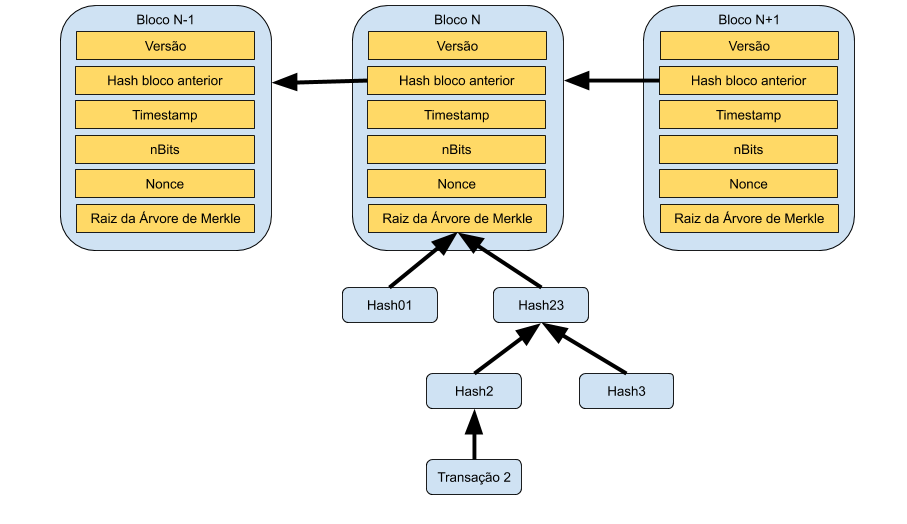
\includegraphics[width=0.9\textwidth]{imagens/esquema_blockchain.png}
\begin{center}
        Fonte: Adaptado de \cite{blockchain:bitcoin_whitepaper} e \cite{blockchain:seguranca_desafios}
\end{center}
\label{fig:esquema_blockchain}
\end{figure}

Na Figura \ref{fig:esquema_blockchain} é mostrada a estrutura do \textit{Blockchain}, como se dá o encadeamento e as características de um bloco individual. 
%
Cada um dos componentes mostrados na parte interior diz respeito a uma variável que porta valores importantes para a construção do bloco, sua identificação e comunicação com a rede.
%
O primeiro campo é a versão do protocolo, e serve basicamente para indicar quais regras de validação devem ser seguidas porque essas podem ser alteradas ou atualizadas com o passar dos anos.
%
O segundo campo compreende o valor de \textit{hash} do bloco anterior e serve, como mencionado anteriormente, para ligar a cadeia. O terceiro campo trata-se do \textit{timestamp} da construção do bloco e por razões óbvias pode levemente variar, uma vez que a assinatura de tempo também é levada em conta no cálculo do \textit{hash} e dessa forma não representará o tempo da finalização do bloco em si.
%
O quarto campo (\textit{nBits}) é responsável por representar o nível de dificuldade de mineração do bloco, ou seja, o quão difícil é gerar um \textit{hash} que seja aceito pela rede. O valor do campo trata-se do número de bits que devem ser iguais a zero no início do \textit{hash} proposto como possível solução para o bloco, caso tal condição seja satisfeita, uma solução válida é encontrada.
%
O quinto campo é o \textit{Nonce} que é um número que começa em zero e após cada \textit{hash} inválido criado é incrementado em um, de modo que se possa tentar gerar um \textit{hash} distinto possivelmente válido para o mesmo conjunto de informações \cite{blockchain:mastering_bitcoin}.

%
O último campo é a raíz da árvore de Merkle que é uma das principais estruturas do \textit{Blockchain}, nela cada nó não final terá o conteúdo igual ao \textit{hash} de seus dois filhos. Assim, nós finais representam algum tipo de dado - nesse caso transações - e os nós ascendentes serão o resultado de sucessivas aplicações da função de \textit{hash} até a raiz, que representa a estrutura como um todo \cite{blockchain:capitulo5}.
%
Por sua vez, a árvore de Merkle é uma estrutura particularmente interessante pois permite o armazenamento parcial dos dados sem comprometer a sua integridade, isso se dá devido à possibilidade de não possuir fisicamente certos ramos, porém estes ainda estarem descritos na estrutura graças ao \textit{hash} de seu pai. Portanto, após a criação da árvore e validação do bloco cujo qual ela pertence um outro usuário da rede não precisa armazenar completamente os dados de todas as transações presentes no bloco para que a cadeia faça sentido, é possível guardar apenas a raiz da árvore ou, no caso de uma verificação pessoal de transações, requisitar à rede que envie um certo ramo específico correspondente a uma transação ou até mesmo grupos de ramos com transações. As vantagens trazidas por tal conceito em relação ao espaço de armazenamento necessário são vastas, principalmente quando confrontadas com a crescente quantidade de blocos nas cadeias e o espaço que ocupam \cite{blockchain:seguranca_desafios, blockchain:bitcoin_whitepaper}.

%
Outra característica importante da tecnologia garantida pelo segundo e último campos é a integridade da cadeia e das informações nela contidas. A existência dos dois campos se complementa pois qualquer tentativa de adulteração em uma das transações, graças às propriedades fundamentais da árvore de Merkle, implicariam em mudança nos \textit{hashes} de todos os nós ascendentes inclusive a raiz, o que influencia na construção do \textit{hash} do bloco como um todo \cite{blockchain:arvore_merkle}.
%
Dessa forma, como o \textit{hash} do bloco anterior é utilizado na criação do bloco atual e o mesmo ocorre para o bloco anterior em relação ao seu predecessor e da mesma forma para todos os blocos ascendentes na cadeia, se qualquer informação sobre as transações for modificada em qualquer um dos blocos predecessores, os \textit{hashes} de todos os consecutivos também serão alterados, o que cria um efeito em cascata que ao atingir o último bloco torna simples a verificação de uma tentativa de adulteração dos dados pela simples comparação dos \textit{hashes} \cite{blockchain:bitcoin_whitepaper}.

\subsection{Formas de redes de \textit{Blockchain}}
\label{subsec:blockchain:pub_priv}

Dentre as redes de \textit{Blockchain} existentes há diferentes modelos de funcionamento para cada uma. Esses modelos dizem respeito principalmente à acessibilidade que os usuários tem para com a cadeia e quanto poder eles têm para operar sobre os registros, no que toca a inserção, visualização e conferência dos dados. Essas formas de funcionamento das redes de \textit{Blockchain} são três \cite{blockchain:formas_redes}:
\begin{itemize}
    \item \textbf{Redes públicas:} Nas redes públicas todos os usuários tem acesso à rede de maneira completa, assim qualquer indivíduo ou entidade pode visualizar o conteúdo que está guardado nos registros e por conta própria averiguar a conclusão ou integridade de repasses transacionais. É possível também que estes, uma vez conectados à rede, possuam fundos e possam efetuar transações para outros usuários, assim como participar dos processos de consenso para validação de blocos. O processo de conexão é dado simplesmente pela obtenção de um endereço válido reconhecido pela rede, geralmente disponibilizado aos participantes através de uma carteira digital que pode ser instalada em uma máquina convencional em poucos passos. Exemplos desse formato de redes são o \textit{Bitcoin} e o \textit{Ethereum}, para os quais existem também diversos sites de terceiros que apresentam informações completas à respeito dessas cadeias de maneira estruturada, como o \textit{Blockcypher} \cite{blockchain:blockcypher} e o \textit{Etherscan} \cite{blockchain:etherscan} respectivamente.
    \item \textbf{Redes Privadas:} Em redes privadas, ao contrário das públicas, somente um grupo seleto de usuários têm acesso aos dados registrados e podem ou não possuir privilégios de execução de transações e participação no processo de consenso. Muitas vezes essas redes pertencem somente a uma empresa central que usa as vantagens do \textit{Blockchain} para auditabilidade e controle dos dados da organização, possuindo um conjunto interno de nós aprovados que podem operar sobre a cadeia. Em tais casos, a participação de usuários externos não é permitida, uma vez que também não há interesse em divulgação de dados sensíveis da empresa que podem estar localizados na cadeia.
    \item\textbf{Redes de consórcio}: Uma rede de consórcio representa um meio termo entre redes públicas e privadas. Nesse modelo o acesso aos dados pode ser público ou restritivo - limitado à quantidade de acessos ou de verificação de informações - enquanto o conjunto de nós que operam sobre a rede é restrito a um grupo confiável que não costuma ser grande como em redes públicas. Esse modelo é utilizado geralmente em aplicações que operam entre negócios, de modo que as instituições controlam a rede no que toca o processo de consenso e transações e usuários públicos podem, em algum nível, ter acesso aos dados da rede. Um exemplo conhecido de rede de consórcio é o \textit{Hyperledger Fabric} \cite{blockchain:hyperledger}.
\end{itemize}

A forma de acesso da rede escolhida para o presente protocolo será levantada na Seção \ref{ch:proposta}.

\subsection{Consenso}
\label{subsec:blockchain:consenso}

Existem diversas formas para obtenção de consenso em redes de \textit{blockchain}, estas independem dos modelos de rede citados na seção \ref{subsec:blockchain:pub_priv} e podem variar de acordo com a necessidade de cada cadeia. A grande diferença nos métodos de consenso reside principalmente na forma de escolha de quem minera o bloco e como esse processo acontecerá.

%
Nas redes públicas de \textit{blockchain} o processo de consenso comumente utilizado é o \textit{Proof of Work}. Os participantes devem provar sua identidade através de um extenso uso computacional para gerar um bloco, o primeiro a conseguir tal objetivo é considerado o criador. Esse algoritmo começa com o \textit{pool} de transações, no qual residem todas as transações efetuadas, porém ainda não confirmadas. Nela os usuários que decidiram participar do processo de mineração escolhem um conjunto de transações, verificam-nas e então constroem uma árvore de Merkle. Ao possuir o \textit{hash} da raiz da árvore o processo de mineração em si pode começar, para tal, o minerador tenta criar um hash que compreende todo o bloco e que respeita o nível de dificuldade imposto pela rede (\textit{nBits}, Seção \ref{subsec:blockchain:specs}), ou seja, que começa com a quantidade de zeros estipulada. Inicialmente o valor do \textit{Nonce} começa zerado e se a primeira tentativa de criar o \textit{hash} não alcança o resultado necessário este deve ser refeito, agora com o valor de \textit{Nonce} incrementado em um e o mesmo acontecerá para cada resultado mal sucedido da função de \textit{hash} \cite{blockchain:capitulo5, blockchain:survey_bitcoin}.
%
Esse processo de tentativas de \textit{hash} é realizado simultaneamente por todos os usuários e como as características referentes ao \textit{timestamp}, transações e ordem das mesmas na árvore provavelmente irá variar entre eles, como resultado emerge uma corrida que possui chances teoricamente iguais para todos os participantes, tendo em vista que por tratar-se de um algoritmo estocástico a solução correta pode tanto ser encontrada na primeira ou na última tentativa executada.

%
Na prática, quanto mais poder computacional um usuário ou grupo de usuários - no caso de uma \textit{mining pool} - possuir (\textit{i.e.} quanto mais rápido se consegue testar as soluções) maiores são as chances de que o bloco seja minerado por tais entidades. Eventualmente o valor do \textit{Nonce} testado por um usuário pode chegar ao seu máximo - no \textit{Bitcoin} são reservados 32 bits para esse campo, o que equivale a cerca de quatro bilhões de possíveis valores não negativos - impossibilitando o minerador de continuar o trabalho. Para resolver esse problema existe outro valor chamado \textit{extraNonce} que reside no nó mais a esquerda da árvore e que deve ser incrementado em uma unidade toda vez que o número de tentativas do \textit{Nonce} original acaba \cite{blockchain:mastering_bitcoin}. 

Em redes que utilizam o \ac{PoW} o valor do campo \textit{nBits} que representa a dificuldade de mineração é aumentado de maneira recorrente dentro de um certo intervalo de tempo. Essa ação é tomada para acompanhar a evolução do hardware, de modo a contrabalancear o poder computacional que aumenta constantemente. Esse processo, entretanto, gera custos energéticos altos, um problema enfrentado em diversas áreas da computação e que representa perdas econômicas e possivelmente ambientais devido às fontes dessa energia. Para contrapor esse obstáculo foram propostas outras formas de consenso menos dispendiosas e prejudiciais.

%
O \ac{PoS} trata-se de uma forma de atingir consenso que baseia-se na quantidade de fundos que os participantes tem daquela moeda, assim usuários mais abastadas terão probabilidades maiores de serem escolhidos para minerar os blocos porque acredita-se que não seria do interesse deles sabotar a rede sobre a qual investiram uma quantidade considerável de recursos. Então para escolher o participante minerador é feito um sorteio ponderado pela porcentagem de patrimônio na rede e o escolhido será o único encarregado do processo de mineração. 
%
O \ac{PBFT} é uma forma de consenso baseada na tolerância de falhas bizantinas e trata-se basicamente de um sistema de votação, comportando até 1/3 de nós maliciosos e necessitando que todos os nós da rede sejam conhecidos. O \ac{DPoS} é uma forma de consenso derivada do \ac{PoS} porém trata-se de uma democracia representativa, ou seja, os detentores de fundos na rede delegam nós para participarem do grupo responsável pelo processo de mineração, diminuindo assim, o tempo necessário para validar os blocos graças ao menor número de participantes envolvidos no processo \cite{blockchain:survey}. 

%
Existem também formas alternativas como: \ac{PoB} na qual os usuários devem gastar ou, como sugerido pelos criadores, "queimar" moedas para receberem chances de minerar um bloco, o que equivaleria ao gasto realizado para comprar \textit{hardware} em redes baseadas no \ac{PoW} porém, graças ao algoritmo empregado, não há necessidade de grande poder computacional para a criação dos blocos \cite{blockchain:PoB}; \ac{PoC} é uma forma de consenso baseada no espaço em disco que um usuário aloca para provar sua identidade \cite{blockchain:origem_PoC} e mais especificamente, no contexto das criptomoedas, um usuário dedica tempo inicial para criar um conjunto de \textit{hashes} que podem servir como solução para os blocos e povoa parte significativa de seu disco com esses dados. No processo de consenso os \textit{hashes} são recuperados da maneira mais rápida possível para tentar minerar o bloco e obter a recompensa \cite{blockchain:burstcoin_PoC}. Existem outras diversas formas menos exploradas de atingir consenso nas redes de blockchain, por exemplo as desenvolvidas para soluções específicas, como é o caso do trabalho de \citeauthor{blockchain:energia_dc} de \citeyear{blockchain:energia_dc} ou ainda outras apenas propostas no meio acadêmico como a \textit{Proof of Luck} \cite{blockchain:PoL}. A forma de consenso escolhida para o presente protocolo será tratada na seção \ref{ch:proposta}.

\subsection{Transações}
\label{subsec:blobkchain:transacaoes}

Para abordar o conceito das transações nas redes de \textit{Blockchain} será utilizada a arquitetura transacional do \textit{Bitcoin}, esta por ser a primeira criptomoeda no mercado e precursora da popularização da tecnologia é tomada como modelo e ponto de partida para a elaboração de novos sistemas desse tipo. Entretanto, a utilização dessa arquitetura não é mandatória e suas características podem e devem ser alteradas para melhor abranger as necessidades do projeto, como no caso do presente protocolo.

%
O modelo de transações do \textit{Bitcoin} funciona como um livro de registro fiscal que possui um conjunto de entradas e saídas para controle de créditos e débitos. Uma transação em si será composta por um conjunto de entradas que apontarão para as saídas de outras transações - encarregadas de assegurar os proventos monetários anteriores - e um conjunto de saídas que serão responsáveis por atribuir o direito de posse desses recursos para um ou mais usuários. Assim, tanto os registros de entrada quanto os de saída representam valores da moeda que, no caso das entradas, devem pertencer ao usuário realizando a transação e no caso das saídas, uma redivisão das entradas para pagamento dos destinatários \cite{blockchain:documentacao_bitcoin}. A Figura \ref{fig:blockchain:transacao} mostra a organização interna de uma transação na rede do \textit{Bitcoin}.

\begin{figure}[ht]
\caption{Esquema de uma transação.}
\centering
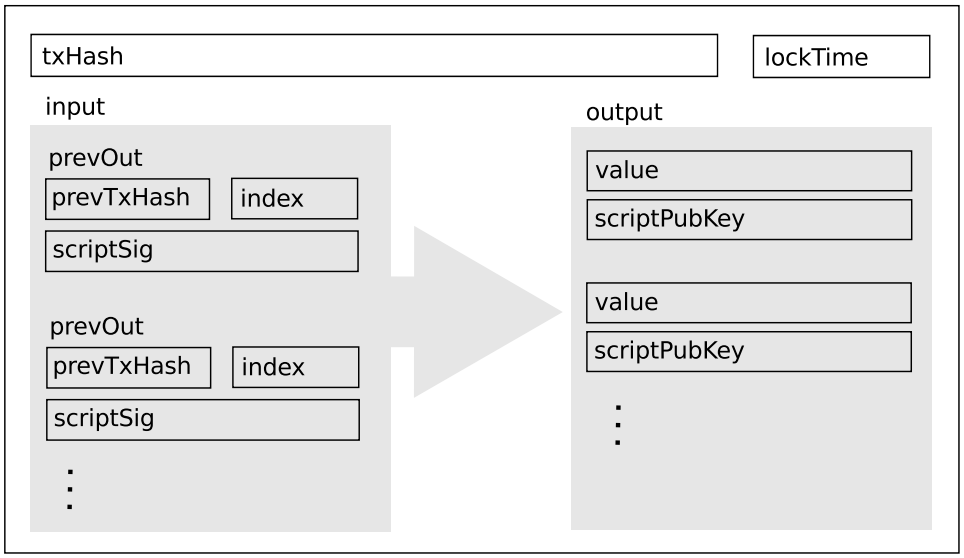
\includegraphics[width=0.75\textwidth]{imagens/esquema_transacao.png}
\begin{center}
        Fonte: Extraído de \cite{blockchain:survey_bitcoin}.
\end{center}
\label{fig:blockchain:transacao}
\end{figure}

A estrutura de uma transação compreende primeiramente o um valor de \textit{hash} para a mesma, responsável por identificá-la na rede. Em seguida há o campo referente ao \textit{locktime} que define quanto tempo - ou quantos blocos confirmados - é necessário esperar antes que as saídas dessa transação possam ser usadas como entrada de uma outra, não sendo um campo obrigatório. A seguir há uma lista não nula de entradas e saídas de transações. Para cada entrada são listados dados referentes ao \textit{hash} da transação anterior e também ao índice da saída dela, cujo valor pode ser utilizado pelo usuário que cria a transação atual, desde que este tenha direito sobre a movimentação do mesmo. Para cada uma das saídas é definido o valor monetário e o \textit{scriptPubKey}, que trabalhará em conjunto com o \textit{scriptSig} das transações que referenciarem essas saídas como insumo. Ambos esses campos são utilizados para a verificação da posse de recursos e cada um deles carrega metade de um \textit{script} da linguagem de programação do \textit{Bitcoin} destinada a esse fim (retomada na Seção \ref{sec:blockchain:smart_contracts}).

%
%
%refazer o parágrafo seguinte, falta clareza
%
%
Quando uma transação deseja utilizar certa saída de outra, é necessário preencher o campo \textit{scriptSig} com a chave pública e uma assinatura que servirá de certificado da chave privada do usuário que reivindica a propriedade. Então, se a execução do \textit{script} contido no \textit{scriptPubKey} da saída, utilizando os parâmetros contidos no \textit{scriptSig} resultarem em uma \texttt{verdade} assume-se que esse usuário é dono das moedas e pode gastá-las. Esse fato pode ser confirmado como verdadeiro porque o usuário que escreve o \textit{script} da saída inclui o endereço de seu destinatário. Então, quando acontece a execução são usadas as duas informações presentes nos parâmetros para construir o endereço público do destinatário e este é comparado com o endereço previamente armazenado na saída. Se a comparação for verdadeira, então a movimentação é aprovada.
%
O conjunto de saídas de transações ainda não gastas de um usuário é chamado de \ac{UTXO} e para que uma nova transação seja aceita é preciso que suas entradas necessariamente referenciem \acp{UTXO}. Os nós que decidem participar dos processos de mineração normalmente mantém um registro dessas transações não utilizadas na memória principal, além do habitual registro em memória secundária. As saídas de transações que já foram referenciadas e que consequentemente tiveram seus fundos utilizados por algum usuário são chamadas de \ac{STXO} - saídas de transação gastas - e dessa forma não podem mais ser referenciadas por nenhuma nova transação e, caso essas tentem, reprovarão no processo de validação.
%
A conexão de entradas e saídas de transações gera diversos fluxos para as moedas e estes eventualmente devem começar em algum lugar. O ponto de partida de um fluxo de transações é sempre uma transação especial que insere novos \textit{Bitcoins} na rede quando um bloco é minerado, essa transação é chamada de \textit{coinbase transaction} e não possui nenhuma entrada de outras transações. O valor da recompensa dessas transações no começo da rede equivalia a 50 \textit{Bitcoins} e é reduzido pela metade, desde então, a cada 210.000 blocos validados. Outra peculiaridade é o tempo de espera, são necessários ao menos 100 blocos confirmados para que uma \textit{coinbase transaction} possa ser gasta \cite{blockchain:survey_bitcoin}.

%
Um outro tipo de recompensa dada para o usuário que minera o bloco é um valor chamado \textit{transaction fee} que, como o nome sugere, trata-se de uma taxa que é paga ao usuário que minera o bloco vindo da diferença entre as entradas e as saídas das transações. Para tal, o valor total das entradas deve, obrigatoriamente, ser maior ou igual ao valor total das saídas de modo que a existência dessa taxa seja possível.

Para o protocolo proposto, as transações podem assumir diferentes formas e representar objetivos de transferência diferentes, esses conceitos serão apresentados na Seção \ref{ch:proposta}.

\subsection{Carteira digital e cliente do usuário}

Para que um usuário tenha acesso a uma rede  de \textit{Blockchain} é necessário que ele possua um endereço nessa rede que seja reconhecido por todos os participantes e que seja passível de verificação no caso da realização de transferências. Tal endereço consiste unicamente de um par de chaves privada e pública, sendo a primeira um número aleatório de 256 bits e a segunda o resultado do uso da primeira como parâmetro de multiplicação no modelo de criptografia \ac{ECDSA}. A chave privada é costumeiramente gerada através de uma carteira digital, que também é responsável por armazenar esses dados - pois em caso de perda da chave privada, o conjunto de moedas guardado pela respectiva chave pública também se perde - para o uso, possíveis migrações para outro dispositivo ou mudança de conta. Aconselha-se aos usuário que troquem seu conjunto de chaves periodicamente, preferivelmente a cada nova transação, de modo a evitar possíveis ataques de descoberta de identidade ou comparação de chaves públicas. Para tal fim, há um histórico de desenvolvimento de modelos de carteiras que que gerem múltiplas chaves. Nos primórdios eram usadas carteiras randômicas, que geravam aleatoriamente um conjunto de n chaves privadas, sendo que todas deveriam ser armazenadas para a possibilidade de migração. O segundo modelo foram as carteiras determinísticas, que geravam uma primeira chave aleatória e posteriormente criavam novas a partir dela, sendo preciso apenas armazenar o dado inicial para que fosse possível refazer todo o processo de computação da criação das chaves posteriores. O terceiro modelo e mais usado atualmente são as carteiras determinísticas hierárquicas, que assemelham-se as suas predecessoras na geração de um dado inicial e reconstrução das gerações, porém gera novas chaves em uma estrutura de árvore, que possui certas vantagens principalmente nos âmbitos da quantidade de chaves diversas que podem ser geradas e no compartilhamento das mesmas (\textit{e.g.} no caso de diferentes endereços sob o domínio de uma mesma entidade ou empresa, destinados a possíveis departamentos ou funcionários).

%
Outro papel fundamental da carteira é agir como cliente para o usuário e atuar como ponto de entrada na rede, no qual muitas tarefas importantes são abstraídas. Nelas, a criação de novas transações se apresenta através de uma interface gráfica para o usuário, o que facilita a escrita e o entendimento, diminuindo a probabilidade de ocorrência de erros. As chaves muitas vezes são mostradas também de maneira formatada, através do uso de mnemônicos, simplificando o processo de armazenamento em meios não necessariamente digitais. Outras funções de nível mais baixo como mensagens de aviso e requisição para outros nós, bem como a escolha das saídas de transações disponíveis para serem utilizadas como entradas para novas transferências são todas tarefas administradas pelas carteiras.

%
Existem ainda, diversas implementações de carteiras independentes e com diferentes funcionalidades quando comparadas às opções nativas ou padrão da rede. Essas também voltam-se para diferentes dispositivos e plataformas, expandindo o poder de escolha e personalização dos usuários na maneira de se relacionar com a rede. Por fim, muitas \textit{Blockchains} fornecem também bibliotecas para o desenvolvimento de novas carteiras, de modo que empresas ou até usuários criem soluções que se adéquem perfeitamente às suas necessidades.


\section{Contratos inteligentes}
\label{sec:blockchain:smart_contracts}

Contratos inteligentes são um conceito que precede o surgimento das criptomoedas e que define uma espécie de regulamentação digital responsável por registrar regras que as partes envolvidas em um acordo legal devem cumprir, estabelecendo punições específicas para diferentes formas de infrações legais. Um contrato inteligente é autônomo na execução e consequentemente na imposição das normas contratuais sobre os envolvidos, representando uma abstração virtual de contratos legais firmados no mundo real \cite{smart_contracts:szabo}. Um exemplo interessante, também proposto por  \citeauthor{smart_contracts:szabo} em \citeyear{smart_contracts:szabo}, é o de um contrato inteligente que regulamentaria a segurança no uso de um veículo. Nesse contrato, algum tipo de imposição física limitaria o uso do automóvel somente ao proprietário, graças à confirmação de uma chave digital criptográfica e se qualquer usuário que não o dono - ou conjunto de donos - tentasse utilizar o veículo, este não obteria êxito. Se por algum motivo esse veículo estivesse alienado como garantia à uma forma de empréstimo, o não pagamento das parcelas ou até mesmo a morte do dono acarretaria na execução do contrato e na transferência automática do direito de posse e utilização do bem ao banco ou instituição responsável pelo empréstimo, sendo tomadas as devidas precauções para não realizar o descrédito da posse em situações críticas (\textit{e.g.} o usuário está utilizando o veículo). Dessa forma, houve uma punição imposta pelo contrato ao usuário em débito, representada pela remoção de seu direito de posse e transferência para a entidade credora. Torna-se portanto simples o entendimento das obrigações das partes, manutenção de rotinas e as punições desferidas sobre os infratores do contrato.

%
No contexto das criptomoedas especificamente, um contrato inteligente possui as mesmas características da definição geral, porém opera exclusivamente sobre transações e movimentação de dados transacionais, servindo como maneira de executar operações mais complexas divisão e retenção de fundos, por exemplo \cite{blockchain:mastering_bitcoin}. Quando ocorre a invocação de um contrato inteligente, no caso da máquina de estados distribuída que é a rede de \textit{blockchain}, este deve ser executado por todos os participantes para garantir a consistência dos registros em todas as cópias da cadeia. Da mesma forma que o modelo transacional, diferentes redes implementam diferentes formas de contratos inteligentes, ou até não os implementam de forma alguma. O Hyperledger Fabric, que trata-se de um \textit{framework} para o desenvolvimento de \textit{blockchains} privadas ou de consórcio, voltadas para comunicação entre diferentes companhias utiliza um modelo de \ac{SC} que além das definições básicas ainda implementa conceitos relativos ao seu meio específico. Características relacionadas a modelos de negócio, \textit{chaincodes} para agrupar contratos baseando-se em grupos de execução para fins semelhantes, políticas de responsabilidade de empresas sobre as transações geradas por \ac{SC} entre outras são modelos únicos implementados por esse \textit{framework} \cite{smart_contracts:hyperledger_fabric}. As criptomoedas mais populares, \textit{Bitcoin} e \textit{Ethereum}, possuem versões menos focadas em nichos específicos do mercado, representando em seus contratos apenas transferências de moedas, cada implementação tendo suas peculiaridades que acarretam em vantagens ou desvantagens em relação a certos aspectos.

\subsection{Contratos no \textit{Bitcoin}}

Na rede do \textit{Bitcoin}, que novamente por ser a primeira criptomoeda funcional introduziu o conceito desse modelo, os contratos são implementados por meio da linguagem \textit{Script} (mencionada na Seção \ref{subsec:blobkchain:transacaoes}) que tem sua utilização fundamentada na verificação de propriedade de fundos monetários que pode ser feita de diversas formas. Essa linguagem é bastante simples - quando comparada as linguagens de alto nível que circulam pelo mercado nos dias presentes - e baseia-se em uma pilha para armazenamento das informações, podendo resolver todas as classes de problemas que um autômato finito com pilha satisfaz. Essa característica foi propositalmente definida como uma escolha de arquitetura por razões de segurança e consistência da cadeia, porque uma vez operando sobre um ambiente distribuído e não necessariamente confiável há necessidade de que seja possível prever o estado da execução de um contrato e que o mesmo seja coerente e alcançável por um conjunto amplo de usuários e possivelmente diverso em \textit{hardware}. A \textit{Script} funciona através de operações que adicionam e retiram dados da pilha e operam sobre esses até que essa encontre-se vazia, assim é possível criar programas que embora simples, realizam com perfeição as necessidades da rede. Os \textit{scripts} são escritos de maneira personalizada e adicionados no campo \textit{scriptPubKey} de cada saída, sendo executados mediante a conferência da validade de uma transação e utilizando como parâmetro o \textit{script} que é armazenado no campo \textit{scriptSig} da transação que a consome \cite{blockchain:documentacao_bitcoin}.

%
Existe um conjunto de \textit{scripts} padrão que realizam ações recorrentemente necessitadas por usuários e que atendem a objetivos diferentes. Transações que utilizam formas verificação do conjunto de \textit{scripts} padrão tem a certeza de que não serão negligenciadas por potenciais mineradores. \textit{Scripts} personalizados, entretanto, podem facilmente fazer com que suas transações não sejam tomadas como participantes em blocos candidatos para mineração \cite{blockchain:mastering_bitcoin}. \textit{Scripts} padrão são responsáveis por diferentes formas de verificação e dentre estas estão: 
\begin{itemize}
    \item \textbf{Pay-to-Pub-Key-Hash (P2KH):} é tratado como se fosse o algoritmo padrão para a verificação de posse e quando é executado simplesmente confere se a assinatura e chave pública fornecidas no \textit{scriptSig}, ao serem submetidas à função de \textit{hash}, geram o endereço correspondente ao escrito no script de trava da saída.
    %
    \item \textbf{Pay-to-Multisig (P2MS):} Esse \textit{script} é utilizado para travar uma transação com um conjunto de $n$ chaves públicas, de modo que seja necessário um subconjunto $m$ de assinaturas para liberar a utilização dos recursos por parte de uma transação \cite{blockchain:mastering_bitcoin}. Um exemplo de uma possível utilização desse script seria o conceito de contas conjuntas, onde é necessária a aprovação de todos os titulares para que se possa mover fundos da conta para terceiros.
    %
    \item \textbf{Pay-to-Script-Hash (P2SH):} Através dessa forma padronizada torna-se possível que um usuário A transfira recursos para um usuário B e que embora o primeiro seja responsável por escrever a transação, o \textit{script} de travamento seja escrito por B. Como é B quem deve realizar o destravamento não há nenhum problema em tal modelo e podem haver situações em que seja coerente, do ponto de vista de B, a existência de algoritmos mais complexos ou completos para a liberação das moedas \cite{smart_contracts:learn_me_a_bitcoin}.
    % O funcionamento, dessa forma, começa com B enviando o hash do \textit{script} que deseja no travamento para o usuário A. Esse então, simplesmente adiciona-o ao \textit{scriptPubKey} com outras operações de verificação e movimentação da pilha embutidas com o único propósito de comparação com o script de destravamento para que, obviamente, não hajam adulterações no resultado esperado. Quando o usuário B deseja usar a transação ele povoa o \textit{scriptSig} com o script que ele enviou ao usuário A junto aos parâmetros necessários para a sua execução. Esse algoritmo é então adicionado à pilha e uma cópia desta é feita. O scriptPubKey é então executado criando uma
    \item \textbf{OP\_RETURN:} Essa operação padronizada é relativamente recente e foi adicionada ao protocolo no ano de 2014 \cite{smart_contracts:bitcoin_0.9} e tem como principal objetivo fomentar a possibilidade do armazenamento de dados não relacionados à transações monetárias na cadeia, tópico que até então gerava discussões desde que o momento em que certos usuários criaram transações substituindo o \textit{scriptPubKey} por dados não relacionados ao modelo, como imagens ou \textit{hashes} de documentos para comprovação de existência. Tal prática criava transações "fantasma" na cadeia que nunca poderiam ser gastas por conter um \textit{script} inválido \cite{blockchain:mastering_bitcoin}. No modelo atual quando uma transação atribui ao algoritmo de travamento a opção \textbf{OP\_RETURN} esta não pode mais ser utilizada como \textit{input} de nenhuma outra e dessa forma, quaisquer valores que foram adicionados à transação são perdidos. O restante do espaço que anteriormente seria destinado para parâmetros e operações do \textit{script} destina-se para armazenamento de dados brutos que não possuem significado ou são interpretados pelo protocolo \cite{smart_contracts:learn_me_a_bitcoin}. É importante ressaltar, entretanto, que não é recomendado o armazenamento de informações não relacionadas à moeda na cadeia do \textit{Bitcoin} por forçar o armazenamento desnecessário de arquivos não importantes para a rede  \cite{smart_contracts:bitcoin_0.9}.
\end{itemize}

Há também uma versão mais simples e anterior ao P2PKH que é o P2PK, que por ser um tanto quanto primitiva em comparação com sua sucessora não foi abordada em detalhes. No que toca os algoritmos padronizados para as transações no \textit{Bitcoin} há possibilidade de inclusão de novas formas a cada atualização, o que diversifica as possibilidades de utilização da rede e dos casos do mundo financeiro que ela pode atender. 

\subsection{Contratos no \textit{Ethereum}}

O \textit{Ethereum} foi a rede que oficialmente introduziu ao mundo o conceito de contratos inteligentes como é conhecido hoje, ou seja, contratos que podem representar uma gama quase ilimitada de possíveis situações de movimentação financeira. O grande fator responsável pelas possibilidades de utilização do \textit{Ethereum} é que seus contratos inteligentes são desenvolvidos em linguagens Turing-Completas, dessa forma podendo resolver qualquer problema que uma Máquina de Turing consegue, representando um poder computacional muito maior do que a linguagem \textit{Script} do \textit{Bitcoin} \cite{blockchain:capitulo5}.

%
Embora o Ethereum seja reconhecido principalmente por sua rede de criptomoedas a proposta formal do mesmo é ser uma máquina de estados transacional de fins genéricos. A própria arquitetura da cadeia do \textit{Ethereum} é bastante diferente do \textit{Bitcoin}, tomando como base um modelo de "balanço de contas" e transações sequenciadas, em oposição ao modelo de "transações não gastas (\ac{UTXO})" usado para especificar o estado de um usuário no \textit{Bitcoin}. Outro fator de diferença entre as duas redes é a forma como elas lidam com os endereços ou contas, sendo que no \textit{Bitcoin} apenas usuários possuem endereços e dessa forma, apenas usuários podem ser referenciados como destino de transações. No \textit{Ethereum} há dois tipos de contas: as \acp{EOA} são contas pertencentes a usuários e, portanto, possuem um par de chaves pública e privada e tem a capacidade de criar transações e movimentar fundos através delas, bem como invocar contratos. As \textit{contract accounts} são contas que não possuem chaves privadas e não pertencem a nenhum usuário, existindo apenas para dar sustento aos códigos de contratos inteligentes. Essas contas também possuem a habilidade de realizar transações de moedas. Quando um usuário deseja executar um contrato inteligente na rede do Ethereum, é necessário que ele referencie uma \textit{contract account} como destinatária. Isso fará com que o contrato seja executado como especificado na transação - pois há campos destinados apenas a transmissão de dados e parâmetros para execução de contratos - pela \ac{EVM} \cite{blockchain:mastering_ethereum}.

%
A \ac{EVM} trata-se de uma máquina virtual que possui o intuito de abstrair um ambiente de execução alheio ao \textit{hardware} para o processamento dos \textit{bytecodes} referentes ao código do contrato compilado. Com a chamada de um contrato, todos os usuários que validarem a sua execução invariavelmente executarão o código na \ac{EVM}, esta possuindo um conjunto de estruturas para armazenamento de memória temporária e permanente para contribuir com o estabelecimento do consenso global.
%
Ao que toca os contratos, por serem Turing-completos, não é possível prever o estado final de dada execução nem mesmo os caminhos que serão tomados para alcançar tal estado. 
%
Portanto, usuários diferentes poderiam executar com sucesso um mesmo contrato com números completamente diferentes de iterações e possíveis saídas distintas.
%
No contexto de ambientes confiáveis distribuídos, essa característica pode tornar-se um empecilho por possibilitar a existência de conjuntos de dados distintos em pontos diferentes da rede.
%
Para contornar esse problema o \textit{Ethereum} faz uso de um conceito chamado \textit{gasLimit}, que é responsável por determinar a quantidade máxima de iterações que poderão ser executadas na computação de uma transação ou contrato pelos usuários na \ac{EVM}.
%
Cada tipo de instrução na linguagem possui um custo diferente em \textit{Gas} e na criação da transação deve ser especificado também um campo denominado \textit{gasPrice}, que compreende o preço que o usuário responsável pela transação está disposto a pagar por cada unidade de \textit{Gas} utilizada em seu processamento. Se eventualmente a quantidade de \textit{Gas} acaba o processamento é interrompido e o estado da execução naquele momento é considerado o final. Se a computação não usou toda a quantidade delimitada no \textit{gasLimit} o valor que sobra é ressarcido ao criador, ao passo que os valores utilizados são pagos ao nó que minerar a transação. Assim, quanto maior o \textit{gasPrice} definido na transação, maiores são as chances de que essa transação seja incluída em um bloco, já que uma quantidade maior de mineradores irá incluí-la no bloco que tentam minerar \cite{blockchain:ethereum}.

Todos os dados apresentados neste capítulo servem como base e fonte de estudo para o desenvolvimento e justificativa das escolhas para a presente proposta, apresentada no Capítulo \ref{ch:proposta}.